\section{System Design}

In this section, we discuss the design of \dbltr{}, our role-based debloating system. 
\dbltr{} consists of data processing, code rewriting (i.e., debloating), and content-delivery steps, making up a full debloating pipeline. 
We evaluate the performance of \dbltr{} on the usage traces collected through our user study. 
Initially, \dbltr{}'s data-analysis step processes the code-coverage traces from web application users and identifies clusters of users with similar behavioral patterns. 
It then produces debloated copies of web applications customized to the needs of each cluster. 

Figure~\ref{fig:system_architecture} shows the end-to-end architecture of \dbltr{}. 
First, we review Step 1 in Section~\ref{sec:debloating}, which consists of analyzing the behavior of users, clustering them into roles and producing the debloated applications for each group of users with similar behavior. 
Then we discuss the design of \dbltr{}'s content delivery modules (Steps 3-7) in Section~\ref{sec:content_delivery}. 
%the technical details of our login detection module is available in Section~\ref{sec:content_delivery}. 

\subsection{Processing the code-coverage information and debloating}
\label{sec:debloating}

We extract the list of file and line coverage information for all users of each web application. 
Next, we identify clusters of users that performed similar tasks. 
In order to cluster similar users together, we train an unsupervised clustering model based on source code features from the users' code-coverage.  

\subsubsection{Data preparation and clean up}

Some web applications (e.g., Magento) create temporary PHP files for caching purposes. 
Other interactions with the web applications such as installing a new module can also result in the introduction of new PHP code. 
For our debloating scheme, we consider an application in a stable state (i.e., we assume that all the required plugins and modules are already installed prior to debloating). 
Therefore, we perform a cleanup step through which we remove references from code-coverage traces that point to non-existing files in the original version of the applications. Our cleanup step will effectively remove newly installed modules during the user study experiments, but will keep the code in the original application that enables users to install new modules. 

\subsubsection{Vectorizing code-coverage} 
\dbltr{} extracts a list of features representing the usage profiles from the code-coverage traces. 
Most commonly, web application source files are partitioned under directories that indicate the feature they implement. 
Moreover, for external dependencies (i.e., composer packages), the file-path includes the name of the module that the files belong to. 
The same holds true for namespaces, class names and function names in that they usually represent the underlying feature that they implement. 
\dbltr{}'s clustering does not need the naming conventions of the web application modules to be meaningful, as long as the naming scheme can uniquely represent the underlying feature that is being used. 

\dbltr{} extracts file names, active namespaces, used classes, and invoked functions from the code-coverage traces.  
These features are effective indicators of the functionality corresponding to each user's code-coverage. 
We then map each feature to a unique representation in a binary feature space. 
Based on these features, we cluster the code-coverage of users using unsupervised clustering algorithms, and optimize the number of clusters (i.e., roles) to produce the best debloating (i.e., highest number of removed functions across roles). 
\dbltr{} then produces the following artifacts:

\begin{itemize}
    \item $N$ debloated variants of web applications, where $N$ is the number of roles that optimizes the debloating by grouping users with similar behavior together. 
    \item Configuration files for the reverse-proxy and the web servers to host the debloated web applications in a containerized environment. 
    \item Database with the mapping of users to roles.
\end{itemize}

\subsubsection{Measuring code-coverage similarity}
Unsupervised clustering requires a measure for similarity between the data points (i.e., code-coverage of users). 
We use the Jaccard similarity coefficient to measure how dissimilar the code-coverage of two users are, and use it as the distance metric in our clustering. 
Under this scheme, we assign the distance of zero to users with identical code-coverage. 
Similarly, we assign a distance of one to users with no overlap in their code-coverage. 

\subsubsection{Clustering code-coverage information} We experimented with three different unsupervised clustering algorithms namely, K-means~\cite{Jin2010}, Spectral clustering~\cite{spectralclustering} and DBSCAN~\cite{dbscan}.
The output of the clustering step is a list of roles and the mapping of users to those roles.  

On one end, we build a single role which acts as the baseline for our debloating measurements. 
This role which contains the code-coverage of all users resembles the ``global'' debloating structure of Less is More~\cite{lessismore}. 
On the other end, we can assign a unique role to each user. 
By doing so, each user receives their own uniquely debloated web application which ensures the maximum tailoring of features. 
We argue that the optimal number of roles lies in between these two extremes, such that the debloating metrics are maximized while minimizing the total number of roles. 

% Moreover, as we quantify in Section~\ref{sec:augmented_coverage}, it is beneficial to group users with similar behavior together and minimize the total number of roles since peers can augment each other's code-coverage. 
% This aggregation reduces the likelihood of users running into removed features even in the case of an incomplete training phase (i.e., features that they did not exercise during the training of the system which were subsequently removed but later decided to use them).

After comparing the debloating statistics of different clustering algorithms, we observed that Spectral clustering outperformed the other algorithms. Therefore, we use Spectral clustering in \dbltr{} and report its debloating statistics in the remainder of this chapter. 
Table~\ref{tab:clustering_lloc_comparison} lists the LLOC reduction statistics for all the evaluated clustering algorithms.

\begin{figure}[]
    \centering
    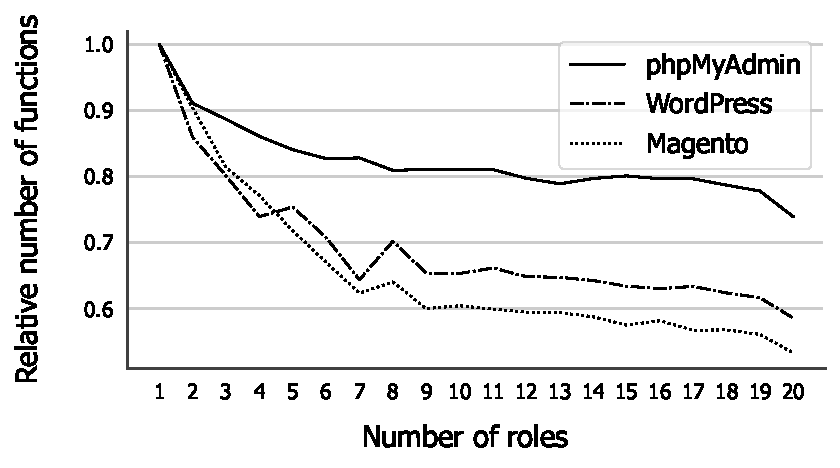
\includegraphics[width=0.8\linewidth]{figures/dbltr/optimalroles_bw.pdf}
    \caption{Reduction in number of functions after debloating for different number of roles compared to ``Global'' debloating (i.e., one role).}
    \label{fig:optimalroles}
\end{figure}

\subsubsection{Determining the optimal number of roles} 
\label{sec:num-clusters}


\dbltr{} determines the optimal number of roles for each web application by using the elbow method~\cite{bholowalia2014ebk}. 
By measuring the decrease in the average number of functions in the debloated copy of the web applications, \dbltr{} chooses the smallest number of roles that produce the highest reduction. 

Figure~\ref{fig:optimalroles} depicts the reduction in the average number of functions remaining in the web applications after debloating based on the total number of roles. 
Given the ways that the 60 administrators used the evaluated web applications during our user study, the optimal number of roles are as follows: six roles for phpMyAdmin, seven for WordPress, and seven for Magento. 

\subsubsection{Debloating the applications} For each role, we merge the code-coverage information for all the users of that role, and then use the aggregate file and line coverage information to identify unused files/functions and debloat them. 
In this step, we first perform file debloating and then debloat functions within the remaining files. 

The process of debloating consists of neutralizing unused files and functions by replacing them with a routine that blocks the further execution of the code. 
By neutralizing unused files and functions, we immediately stop the execution of code paths that invoke the debloated code. 
This immediate termination would prevent the application from executing paths with debloated functions and potentially introducing new bugs. 
Moreover, this allows us to display an error message to the user and log this event for the administrators for further analysis (e.g., in the case of potential exploitation attempts). 

This debloating procedure provides us with \emph{N} copies of the original application, with \emph{N} being the optimal number of roles determined by \dbltr{}. 
Debloated applications for each role cater to the use cases of all their underlying users. 
Lastly, we measure the debloating metrics such as size, CVE, and CAC reduction across the debloated copies of our web applications. 
We discuss these results in more detail in Section~\ref{sec:debloatingresults}.

\subsection{Content delivery}
\label{sec:content_delivery}

The second stage of the \dbltr{} pipeline is responsible for serving the debloated web applications and seamlessly routing users to their underlying debloated web applications. 
\dbltr{} implements a reverse-proxy module based on OpenResty, which is a popular high performance scalable web server that extends NGINX and provides content manipulation APIs through Lua code~\cite{openresty}. 
This is depicted in Figure~\ref{fig:system_architecture} as step 3. 

We implement the login-detection logic as a Lua module for OpenResty. 
This module is responsible for detecting successful login requests, extracting username and session cookie information, as well as storing and retrieving the user-to-debloated-application mappings from the data store.

\begin{table}[t]
    \caption{Minimum, median, and maximum size of debloated applications for optimal number of roles reported as thousands of LLOC.}
    \label{tab:clustering_lloc_comparison}
    \centering
    \begin{adjustbox}{max width=0.8\columnwidth}
    \begin{tabular}{|l|l|lll|}
    \hline
    \multirow{2}{*}{\textbf{\begin{tabular}[c]{@{}l@{}}Web \\ Application\end{tabular}}} & \multirow{2}{*}{\textbf{\begin{tabular}[c]{@{}l@{}}Clustering\\ Algorithm\end{tabular}}} & \multicolumn{3}{c|}{\textbf{K-LLOC}}                                                    \\ \cline{3-5} 
                                                                                         &                                                                                          & \multicolumn{1}{c|}{\textbf{Min}} & \multicolumn{1}{c|}{\textbf{Median}} & \textbf{Max} \\ \hline
    \multirow{3}{*}{phpMyAdmin}                                                          & Spectral                                                                                 & \multicolumn{1}{c|}{32}           & \multicolumn{1}{c|}{39}              & \multicolumn{1}{c|}{42}           \\ \cline{2-5} 
                                                                                         & DBSCAN                                                                                   & \multicolumn{1}{c|}{34}           & \multicolumn{1}{c|}{39}              & \multicolumn{1}{c|}{41}           \\ \cline{2-5} 
                                                                                         & K-means                                                                                  & \multicolumn{1}{c|}{32}           & \multicolumn{1}{c|}{40}              & \multicolumn{1}{c|}{42}           \\ \hline
    \multirow{3}{*}{WordPress}                                                           & Spectral                                                                                 & \multicolumn{1}{c|}{44}           & \multicolumn{1}{c|}{54}              & \multicolumn{1}{c|}{64}           \\ \cline{2-5} 
                                                                                         & DBSCAN                                                                                   & \multicolumn{1}{c|}{47}           & \multicolumn{1}{c|}{59}              & \multicolumn{1}{c|}{64}           \\ \cline{2-5} 
                                                                                         & K-means                                                                                  & \multicolumn{1}{c|}{44}           & \multicolumn{1}{c|}{52}              & \multicolumn{1}{c|}{64}           \\ \hline
    \multirow{3}{*}{Magento}                                                             & Spectral                                                                                 & \multicolumn{1}{c|}{241}          & \multicolumn{1}{c|}{270}             & \multicolumn{1}{c|}{326}          \\ \cline{2-5} 
                                                                                         & DBSCAN                                                                                   & \multicolumn{1}{c|}{251}          & \multicolumn{1}{c|}{275}             & \multicolumn{1}{c|}{310}          \\ \cline{2-5} 
                                                                                         & K-means                                                                                  & \multicolumn{1}{c|}{251}          & \multicolumn{1}{c|}{283}             & \multicolumn{1}{c|}{316}          \\ \hline
\end{tabular}
\end{adjustbox}
\end{table}

The login procedure for web applications consists of a request containing the credentials followed by the server response assigning the authentication cookie to the users in the case of successful login. 
\dbltr{} inspects the request-response pairs for successful login attempts. 
Listing~\ref{lst:lua} demonstrates the authentication detection logic for phpMyAdmin. 
For this web application, a successful login comprises a POST request towards the login endpoint ``/'' or ``index.php'' that receives a 302 HTTP response code which redirects the user to the administration page of the application (Line 2 in Listing~\ref{lst:lua}). 
We extract the username from the POST request with the field name of ``pma\_username'' (Line 4) and then verify through the HTTP response code that we detected a successful login (Line 9). Finally, we extract the session cookie named ``phpmyadmin'' (Line 12) and store this user-to-session-cookie mapping in the Redis data store for subsequent requests. 

During the debloating stage, \dbltr{} produces mappings that directs our OpenResty module to redirect users to specific instances of debloated web applications. 
This information is stored in a Redis data store along with a hashed copy of the session cookie and username mappings extracted by the Lua module. Producing these Lua modules is a simple process for anyone with a basic understanding of web applications who can use approaches such as the Developer Tools of modern browsers to identify the right requests, and form fields. Once authored, these short modules (typically under 20 lines of Lua code and mostly made up of boilerplate code) will be valid for \emph{all} deployments of that web application and will only need to be updated, if the web application changes its authentication logic in a later version. 


% \definecolor{commentsColor}{rgb}{0.497495, 0.497587, 0.497464}
% \begin{lstlisting}[belowskip=-1em, caption=LUA configuration to detect successful logins and extract authentication cookies for phpMyAdmin,label=lst:lua,basicstyle=\footnotesize, float=tp, floatplacement=tbp, language={[5.0]Lua},commentstyle=\color{commentsColor}\textit, numbers=left, xleftmargin=5.0ex, breaklines=true]
% -- phpMyAdmin Username extraction
% if post_params ~= nil and (string.find(ngx.var.request_uri, "/") or string.find(ngx.var.request_uri, "index.php")) 
%   then
%     if post_params["pma_username"] ~= nil then
%       username = post_params["pma_username"]
%     end
% end
% -- phpMyAdmin Successful login detection
% if ngx.var.request_method == "POST" and ngx.var.username ~= "" and ngx.status == 302 then
%   -- Successful login detected extract session cookie
%   for key, value in pairs(cookies) do
%     if string.match(value:lower(), "phpmyadmin") then
%       -- Store cookie value in Redis
% \end{lstlisting}

For subsequent requests containing a valid session cookie, \dbltr{} first queries the username from the data store and then determines the target web server based on the username mapping. 
Steps 4, 5, and 6 in Figure~\ref{fig:system_architecture} depict this process. 
Once the upstream web server is determined, traffic is routed to the corresponding web server. 
Any subsequent log-out requests and timeouts invalidate the session-cookie mapping.